%================================================
%================================================
%================================================
\chapter{Related Work} \label{ch_relatedwork}

%TODO Intro to the chapter
Activity recognition is a cognitive skill that can be considered within perception. 
It deals with the interpretation and understanding of a scene by processing a sensory input and correlate it with domain knowledge to be able to associate it with an activity pattern.

The fundamental concepts to understand the problem of activity recognition lies in Psychology, as this is the science that studies the mind. 
Then, the problem that follows is to replicate this cognitive process into a machine, particularly a robot; this is the focus of study of Artificial Intelligence and Robotics.
The aim of this project is to study the use of ASP in robotics for knowledge processing and reasoning; looking, in particular, to the problem of activity recognition with a mobile robot. 

This chapter presents relevant related work.
First the antecedents of perception in AI are traced to serve as a basis for the rest of the chapter.
Then the problem of activity recognition is briefly reviewed to provide a general overview of the area and also, to locate this project in the \textit{map} of research in the area.
Finally, closely related work is presented to point the current state of the area and exhibit open trends in the area where the current project has possibilities to provide continuity.



% 0 - GENERALITIES
% Perception
% Symbol ground
% Anchoring
% Frame Problem

\section{General antecedents - Perception in AI} \label{ch_LitRev_Perception}

Perception, as a cognitive process, has been studied widely in Psychology.
It refers to the process of organizing and interpreting sensory information so that it has a meaning \citep{King2014Psychology}.
Part of the interest lies in how sensory information is processed by the brain, and which parts of it are essential.
Also relevant, it is the domain knowledge, previously acquired or consulted, that the subject uses to establish a meaning to the sensory input.
Together, the sensory input and the domain knowledge are used to interpret a scene.

%TODO Other interesting examples to discuss later: Plato's Cave, 5 blind men and the elephant, Flatland, Metamorfosis.

Sensory input is important for perception, however, not all the data is equally important to interpret a particular scene and conclusions can still be made, even with partial data.
In \citep{Heider1944_Experimental}, an animated film was created using only moving polygons to demonstrate how the motion of abstract entities could be interpreted by human observers in meaningful ways.
In \citep{Johansson1973_VisualPer}, locomotion patterns of living organisms using visual marks were studied. 
By this mean, the emphasis was put in the qualitative motion description of the marks rather than in the qualitative motion description of the moving body.
Both works show that, even with abstract entities, the human mind is capable to create or associate concepts to them using only a limited amount of information.
Also, that perception is a more complex mental process than just processing sensory data.

In Artificial Intelligence, perception has been studied principally by the computer vision community.
Earlier works can be traced back to the 1960s, as part of the effort to mimic human-like intelligence using visual perception components. The main difference between computer vision and image processing has been the desire to recover the three-dimensional structure of the world from images, and to use this as a stepping stone towards full scene understanding \citep{Winston1975_PsyCV}. 


One of the first works in 3D reconstruction from a single image is found in \citep{Roberts1963_PhDThesis}.
The developed system was able to reconstruct geometrical bodies with flat surfaces by recognizing the borders of the bodies in the scene and later analysing the shades of their visible surfaces.
%TODO Maybe include Adolfo Guzman Arenas work here. +-
In \citep{Barrow1971_RelatDesc} object recognition was studied by decomposing an image into regions and describing the spatial relations between them, in a more qualitative, rather than the traditional quantitative pixel-based approach.

Since the early 1970s, the \textit{block's world} was used as a test scenario for intelligent systems, particularly regarding knowledge representation, reasoning and planning.
In the block's world, an initial state $A$ and a desired state $B$  of the environment are given.
The goal is to autonomously generate a plan to transform $A$ into $B$ by the manipulation of the blocks.
One important characteristic of the problem is that requires a symbolic description of the scene.
The problem was used as a test case for the robot Shakey \citep{Nilsson84_Shakey}.

%Finally, during the 1980s an approach to perception with emphasis in action feedback became popular
%TODO Complete Active Perception.
During the late 1980s, the concept of \textit{active perception} emerged to emphasize the role of control during the sensing phase \citep{Bajcsy88_ActivePerception}.
This is, the capacity to adapt the sensing strategy by considering the data interpretation and the goal task.
It is clear that a robot is an active agent, so it is desirable to take advantage of active perception strategies.
In the context of activity recognition with a mobile robot, an active perception strategy would be to close the control loop by directing the robot actions with the former results of the activity recognition system, to improve the data collection and, eventually, improve current and future conclusions.


%TODO Need to mention QSR.
%TODO Need to mention KRR (ASP, DL, Ontologies, Naive Ph, etc.).


\section{Activity Recognition} 
% Emphasis in the taxomony of the area. I will only describe the taxonomy and give examples. I need to finish with describing the branch that fits better the "robotics" approach, and that will be the next section.

Activity recognition is an important research area in the context of automated perception. 
It has many applications as surveillance, inspection, verification, generation of automated reports, etc.
The application will dictate the approach to follow and the kind on sensors that will be required.

Human activities can be classified in different ways.
In \citep{Turaga2008_MaRecHuAcSurv}, two non-exclusive categories are used: actions (performed by a person) and activities (performed by many persons).
One more descriptive categorization has been given in \citep{Aggarwal11_HumanActivity}, separating activities in four classes:

\begin{description}
\item[Gestures] Elementary movements of a person's body part, and are the atomic components describing a meaningful motion of a person. 
E.g. `stretching an arm', `raising a leg'.
\item[Actions] Single person activities that may be composed of multiple gestures organized temporally. 
E.g. `walking', `waving'.
\item[Interactions] Human activities that involve two or more persons and/or objects. 
E.g. `Two persons fighting', `a person eating an apple'.
\item[Group activities] The activities performed by conceptual groups of multiple persons and/or objects. 
E.g. `a football team playing a match', `a group of students making an exam'.
\end{description}

All of these categories require to be able to sense humans with different level of detail.
For example, gestures require specific algorithms (e.g. hand detection, face detection, skeleton tracing, etc.) while long distant pedestrian tracking algorithms may consider persons as \textit{moving dots}.
The type of activities to be recognized will dictate the required algorithms.

In the same fashion, activity recognition approaches can be classified in basis of different factors.

First, regarding the sensors, two approaches can be followed, distant or pervasive. 
The first one observes the scene from the distance as it happens with a CCTV camera or a robot. 
The pervasive approach relies on wearable devices to detect the activity of a person from a first person point of view.

Another possible classification of activity recognition systems focuses on how information is processed.
In \citep{Aggarwal11_HumanActivity} a taxonomy is proposed as shown in Fig. \ref{fig:taxonomy}.  

\begin{figure}[h]
\centering
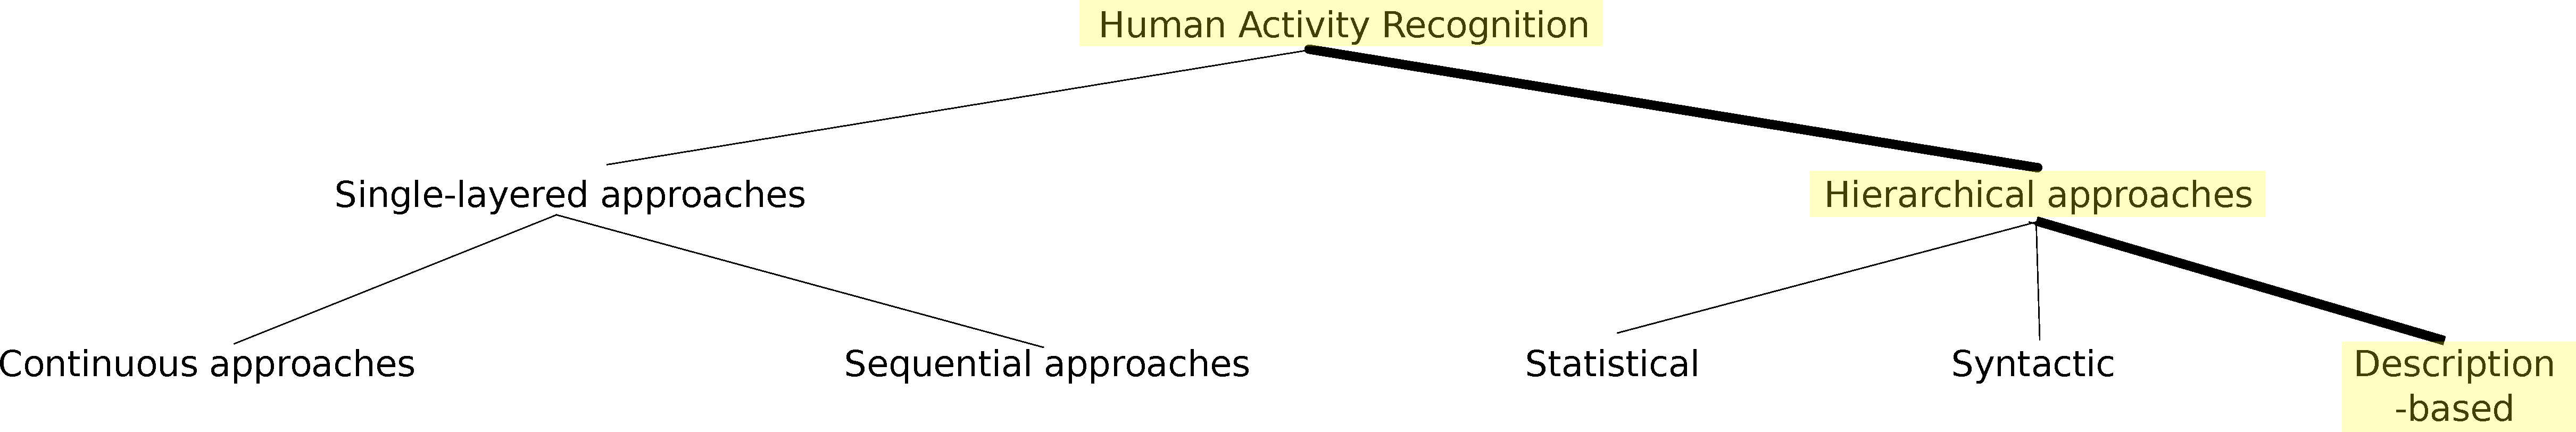
\includegraphics[width=\textwidth]{fig/img_Aggarwal_Taxonomy3.pdf}
\caption{The taxonomy of research in activity recognition described in \cite{Aggarwal11_HumanActivity}. It has been highlighted the branch that follows this project.}
\label{fig:taxonomy}
\end{figure}

\subsection{Single-layered approaches}
They represent activities in terms of raw sensory data\footnote{The original survey \citep{Aggarwal11_HumanActivity} describes single layered approaches as image-based approaches, but it leaves out the systems with other sensing capabilities (e.g. 3D sensors, sonars, GPS, etc.).
However, they can be included too the activities are represented in terms of raw sensory data patterns.}, because of this, the activity descriptions are trained from datasets.

%Sensory data is processed to obtain particular descriptive features of the scene which are compared with known activity patterns. 
%These patterns can be obtained in a supervised or unsupervised fashion (e.g. common occurrences of a specific action). 
%Most of them are based in computer vision and machine learning techniques.

Single-layered approaches are suitable to recognize short-term and simple activities as gestures, movements of the body or simple interactions with objects. 
This is mainly because the amount of sensory data grows very easily and long-term activities would require to process larger amounts of data. 
Also, because activities are not always performed in the same way, even by the same individual.
The shorter the activity, the more accuracy that will be attained.
Finally, this approach is very sensitive to the input sensory data as this will depend on the environmental conditions (e.g. lighting, point of view).


\subsubsection{Continuous approaches\footnote{`Space-time approaches' in \citep{Aggarwal11_HumanActivity}}} % BEFORE: Space-Time approaches

The activities are recognized by analysing continuous sensory data and compare it with an activity pattern.

An activity is represented as a block of data along time where the activity was performed, and it is considered as a whole.
A volume (or hyper-volume) is built by concatenating the sensor readings in time.
The dimension of the data will depend on the sensing capabilities of the system; for example, a video stream would require 3 dimensions $(X,Y,T)$ and a RGBD camera would be able to use 4 dimensions $(X,Y,Z,T)$, etc. %TODO Consider RGB values..., what happens with other dimensions, e.g. temperature?
The sensory input is compared with the activity patterns to measure similarity.
If a threshold is fulfilled, then the activity is labelled.

The advantages of this approach is that it is relatively fast and doesn't require domain knowledge.
On the other hand, these methods have a big dependence of the training data and they are sensitive of the environmental conditions, different sampling rates, discontinuity of the data, the manner in which the activity is performed and the observation point of view. %TODO HOMEWORK: What about interpolating the data in incomplete situations, sometimes seems fair, but in other seems unlikely... again adaptable policies looks interesting.

There are many examples of this approach.
In \citep{Bobick2001_RecHuMovTemp} a video stream of aerobics exercises is analysed by attaching to every pixel a vector indicating the presence and recency of motion. 
Then, the stream was compared online with previously described activities to look for matching. 
In \citep{Ke2007_SpTmpShapeAR}, volumes were built by attaching similar regions of adjacent frames.
Then, the problem was transformed in an object matching problem by comparing the shapes of the volumes (sensory stream and activity patterns).

\subsubsection{Sequential approaches} 
%TODO Go deeper.

Sequential approaches represent activities as a sequence of states. 
A state is a vector of features observed in the scene in a specific instant.
Finally, the sequence is analysed depending on the activity representation.
There are two types of methodologies adopted in sequential approaches: exemplar-based and model-based.

In exemplar-based methods, activities, or a class of them, are represented as a sequence of states. 
Then the sensory input is compared in similarity with the patterns.
An example can be found in \citep{Darrell1993_STGestures}, where states are built from view models.
Templates of activities are from sequences of states associated with a physical change (e.g. rotation and scale).
The dynamics of articulated objects in scene were recognized using the dynamic time warping algorithm (DTW) to the sequence of states.

In model based approaches, the sequence of states is compared with a set of probabilistic models of activities. The models are built assuming a temporal dependence between the states, so the transitions are modelled statistically using hidden Markov models (HMM), dynamic bayesian networks (DBN), conditional random fields (CRF), etc.

The first work to use HMM to recognize activities was \citep{Yamato1992_RecHA_HMM}. They transformed a video stream into a sequence of vectors of image features. Then every vector was transformed to a symbol using vector quantization. Finally, a set of HMMs were created to model the activities, and their parameters were optimized. 

\subsection{Hierarchical approaches}
Hierarchical approaches of activity recognition refer to those where complex activities are represented in terms of simpler ones. 
This kind of representation organizes the activities in multiple layers of complexity and creates, by this mean, a hierarchical structure.
In the lower level, atomic (or primitive) actions are represented which are indivisibles; they are usually recognized using single-layered approaches.

Hierarchical approaches are also adequate to represent activities symbolically, by taking advantage of the multi-layered organization, it is possible to describe describe semantic relations.
By these means, they are less dependant to training data and they can integrate domain knowledge more easily.

Hierarchical approaches can be categorized, by the used methodology for recognition, in: statistical, syntactical and description-based. %TODO Expand.


\subsubsection{Statistical}
They are based in the hierarchical construction of statistical state-based models, such as HMMs, DBNs or CRFs.

First, the activities are defined and organized hierarchically.
In the bottom level, atomic actions defined in terms of feature vectors which are obtained from sensory data.
The sequence of feature vectors is analysed statistically to be able to recognize, this is performed in the same fashion as in single-layered sequential approaches. 
Then, the sequence of atomic actions is considered to be the input observations to recognize the next layer of activities, and the same statistical methods can be used to recognize the second layer of activities.
The procedure is repeated in every layer.

Some disadvantages of the statistical approaches are their difficulty to model the temporal structure of events (e.g. $A$ occurred `during'/`before'/`after' $B$) and also, because of their sequential nature, it becomes harder to handle multiple concurrent tasks.

In \citep{Oliver2002_LayRepHumActRec}, the authors present layered hidden Markov models (LHMMs) for online activity recognition using data from video, sound and keyboard data. 
They divide their system in three layers: the first one is in charge of recognizing features from every source, the second layer trigger short events from the scene, and the last layer is in charge to recognize longer activities. 
The hierarchical approach adopted showed an improved performance when compared with single-layered systems.
The training data is used more efficiently and also, it becomes easier to add more detail on specific activities, i.e. to handle different granularities in the activity descriptions.

In \citep{Liao2007_LIT,Liao2007_HCRFGPSAR}, the authors present studies of hierarchical DBNs and CRFs applied to location-based activity recognition.
The authors use GPS data from mobile devices and domain knowledge from locations to learn and infer routines and activities.
As the sensory input are the spatio-temporal traces of the person, domain knowledge from the locations is considered to add significance to the events. 
For example, a quick car stop can be part of an important activity as leaving the children at school or simply caused by a traffic light.
First they segment spatially the traces by grouping neighbour samples that occur in the same region.
They distinguish two major categories of activities: \textit{navigation} (e.g. walking, driving a car) and \textit{significant} (e.g. work, visit, sleep).
Their model is built, in the lower layer, to classify the segmented tracks in activities (events), by looking at their location and the speed of the subject; and finally, in an upper layer, they use these activities to learn distinctive places (e.g. house, office, etc.).


\subsubsection{Syntactic}
In the syntactical approach, activities are represented symbolically as a set of production rules generating a string of atomic actions which is later recognized using parsing techniques.
Atomic actions are obtained with a single-layered approach, however, in higher layers, recognition is performed symbolically.
Context-free grammars (CFGs) and stochastic context-free grammars (SCFGs) are some of the techniques that have been used to recognize high level activities.

One limitation of this approach is the difficulty to handle concurrent activities, and also to consider unexpected events that are not integrated in the grammar.

An example can be found in \citep{Ivanov2000_RecVisActSCFG}.
The authors aim to recognize complex activities in sequences of video.
Two layers are defined; in the lower level, atomic actions are recognized using HMMs, and in the upper one uses SCFGs.
The adopted approach showed to be able to handle longer time activity constraints and also, to be more robust regarding uncertain detections in the lower level.


\subsubsection{Description-based} \label{sec_description_ap}
This approach represent activities as a hierarchy of events, making emphasis in their spatial, temporal and logical structures.

A complex activity is modelled from de occurrence of its sub-events that satisfies certain relations.
The temporal relation between sub-events is also considered in the representation, Allen's interval algebra is frequently used for this \citep{Allen83_MaintainingKnowledgeTemporal}.
Atomic actions are obtained from sensory data and summarized. %TODO Check

Now to recognize activities the problem becomes a \textit{constraint satisfaction problem}, which is NP-hard.
This approach allows a good integration of additional knowledge sources. 
Particularly, the 

There are many possibilities to treat the problem. In \citep{Nevatia2004_OntoVidEvRep,Ryoo2006_RecHuAcCFG}, CFGs are used to represent activities hierarchically, defining temporal relations between sub-events. 
In \citep{Sridhar10_UnsupervisedLearning}, relevant features from the scene are extracted and their behaviour is represented using qualitative spatio-temporal relations (QSTR), then patterns of activities are learnt using Markov chains.


\section{Description-based activity recognition and robotics}

In this project, the chosen approach to follow is a description-based methodology. 
This section presents relevant related work in this line, and sin the Answer Set Programming (ASP) paradigm for 
Also, here are presented the precedents of activity recognition with mobile robots.

\subsection{Description-based activity recognition}

As mentioned in section \ref{sec_description_ap}, description-based approaches represent activities hierarchically by decomposing complex activities in sub-events.
The representation should also make emphasis in the spatial, temporal and logical structures.
The recognition is performed by obtaining features from scene (spatial, temporal, logical) and creating a scene description as a \textit{list} of facts, then the problem becomes a constraint satisfaction problem, to find the best activity match for these set of observations. 

\subsubsection{Representationof activities}

%Regarding the representation of activities, there are many desired characteristics. 
An activity is represented as a set of \textit{facts} that needs to be fulfilled with the observations.
This is important, because the facts can be used as logical predicates.
These facts act as constraints between the activity patterns and help to discriminate between them, some of them may be more relevant than the others.

The execution of an activity depends on the subject, and even a particular subject doesn't execute the same activity in the same way.
This is the reason why activities are usually defined in qualitative terms, i.e. in a symbolic more human-like manner.
Quantitative descriptions of activities are still interesting, however, they are restricted to specific domains as rehabilitation or sports.

Regarding space, Qualitative Spatial Representations (QSR) are a set of calculus which allow a machine to represent and reason about spatial geometrical entities \citep{Cohn2008_QSRR}, e.g. lines, dots, regions, etc.
They are usually combined with a temporal representation to represent the dynamics of behaviours.

Time can be represented as an instant $t$ or as an interval $(t_1,t_2)$. 
For the instants, simple temporal logic can be used to represent these kind of statements. 
Intervals have been typically treated with two approaches \citep{Fisher2008_TempRepReas}: Interval temporal logics \citep{Moszkowski1983_RDC} and Allen's interval algebra \citep{Allen83_MaintainingKnowledgeTemporal}.

%Interval temporal logics have been typically used in the description of computer, particularly hardware and protocols.
%TODO EXPAND Check the article by Allen

Allen's interval algebra is a calculus for temporal reasoning.
It defines 13 possible relations between intervals, and provides a composition table that can be used for reasoning about temporal descriptions of events \ref{fig:allen}.

\begin{figure}[h]
\centering
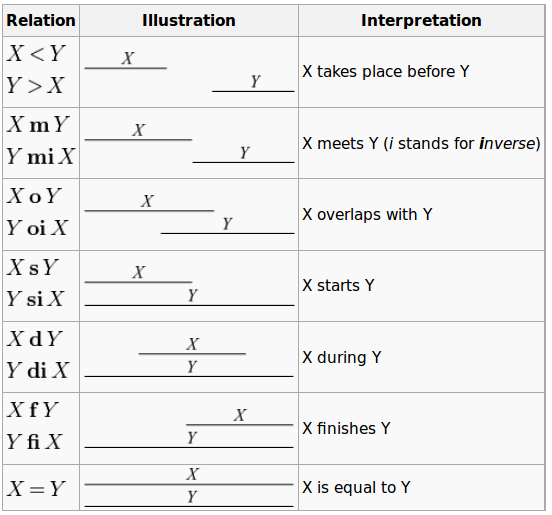
\includegraphics[width=4in]{fig/allen_interval.png}
\caption{Temporal relations of events in Allen's interval algebra}
\label{fig:allen}
\end{figure}


%Tony Cohn
In \citep{Sridhar10_PhD_UnsupervisedLearningEvent}, activities are learnt, in an unsupervised fashion, and recognized from video sequences by reasoning under qualitative spatio-temporal representations (QSTR). 
Objects positions and their trajectories are extracted from scenes and represented in QSTR.
Activities are learnt using a Markov Chain Monte Carlo (MCMC) procedure to find the maximum a posteriori probability (MAP) of candidate interpretations.
This work shows an example of unsupervised learning of activities, using simulated and real examples.
The qualitative approach (QSTR) is robust to changes in the execution of actions and to sensory errors.
Finally, the categorization of activities showed to be reliable in learning functional object categories which provides semantic information from the scene.
On the other hand, some limitations of this work are a fixed point of view and a posterior analysis.
First, the analysis is performed only in short video sequences, and in short activities.
Also, the search space grows very easily as the scene becomes more complex.

%Jay Young
In \citep{Young13_PredcitingSituatedBehaviour,Young14_EffectsTraining}, QSTR are applied to the analysis of multi-agent behaviour in the RoboCup simulation league, particularly in estimating future behaviours. 
Positions, trajectories and orientation of the agents in the scene are described using region connection calculus (RCC), qualitative trajectory calculus (QTC) and the Star calculus respectively. 
Other agent's behaviours are learnt by using a HMM, which is fed with the current observations and a window of previous ones. 
As not all the data is relevant, this is first filtered. 
This work presents a study of activity prediction.
The results show that qualitative representations are more easy to treat general cases of activities and require less training data.
Some drawbacks are that the system posses global information from the environment, and the application domain is restricted.


%\subsubsection{Reasoning}

% Mohan Sridharan & JL Wyatt
% Shiqui Zhang

% Alessandro Saffiotti
% (Cirillo, Pecora, Coradeschi)

% Siskind
% Event recognition

% Benjamin Kuipers


\subsection{Activity recognition and robotics}
A robot is an ideal system to perform activity recognition. 
This is, indeed, a desirable skill for an autonomous robot that will share an environment with people.
The robot needs to be \textit{aware} of the surrounding humans.

Some important challenges to consider with a robot are:

\begin{description}
\item[sensing] Sensing data is usually corrupted because of hardware limitations, presence of statistical noise, discretization by the digitalization process, unstable or moving sensors, unpredictable environment conditions, etc.
The collected data is restricted by the location of robot (there is no omni-presence) and as a consequence the robot will only gather information from the visible parts of the environment, loosing the rest of it.
\item[storage and processing] %Depending on the problem and the followed approach, activity recognition can become a demanding processing task.
Sensory data can grow very easily and its storage and processing becomes a challenge.
Domain knowledge is usually restricted to the field of application, as general knowledge sources are too big to be portable and are only available by online consult.
The algorithms' complexity is usually big in the required problems to solve (e.g. pattern recognition, logic programming, etc.). 
\item[time] Time constraints are relevant in robotic systems as, for many interesting applications, the data cannot be post-processed, i.e. real-time response is required.
\end{description}

During the early years of robotics, much of the effort in the field was put in designing reliable motion planning and control techniques, e.g. \citep{Moravec1983_StanfordCMUCarts,brook-1985:robuslayer:TR}. 
Meanwhile, new advances were also made in fields as computer vision (e.g. optical flow, visual tracking, etc.), knowledge representation and reasoning (e.g. qualitative reasoning, frame languages), and machine learning (e.g. HMMs, decision trees, etc.).
It was until the late 80's and early 90's that robots started facing realistic and non-controlled environments.

One of the first works in activity recognition with a mobile robot can be found in \citep{Kortenkamp1996_RIG,Bonasso96recognizingand}. 
The authors used a monochromatic stereo-vision system mounted on top of a mobile robot for gesture recognition.
They implemented an active approach by dividing the scene in cubic volumes.
Volumes with similar motion vectors are merged and they are chained to a known human model to produce a linked representation of the human.
The angles of the linked representation are compared to a set of previously defined gestures, to label the execution of the gesture.
This work only uses a static representation of gestures within a single layer, and was tested in a scenario where a human points regions of interest to a robot, and the robot gives a response.
The authors point the the consideration of the temporal dimension, group activity recognition and integration with speech recognition as interesting research directions.

As mobile robots started to be used in everyday environments, human robot interaction became more relevant. 
For example, in \citep{Burgard98_ExpMuseumRobot} the authors focused in the problem of motion planning in human environments (a museum). 
However, they point the relevance of human-robot interaction, a robot is not an isolated agent, and humans provide important information about the environment and to be able to complete the task (e.g. giving a tour). 
In future work, the same group studied the problem of human tracking from a mobile platform using particle filters \citep{Schulz01_TrackingMultipleMoving,Schulz03_PeopleTrackSJPDAF} and motion behaviour recognition using the EM algorithm \citep{BennewitzBT02,bennewitz2004active}.
The authors point interesting research open areas in group tracking (instead of individual tracking), particularly the necessity of a flexible approach to handle individual and group tracks of humans and objects at the same time.
Also, as motion patterns have been learnt in a particular environment, an interesting problem is to be able to reuse this knowledge in different scenarios where people show similar behaviours, i.e. a portable gait recognition system.

Human activity recognition also plays a central role in the problem of human-robotic cooperation.
In this context, to achieve cooperation, a robot needs to  be aware of its human partner and integrate itself to the common task in a non-obstructive way.
With this in mind, a robot needs to be able to observe and also to communicate with his human partner.
This requires a sensory approach of activity recognition, but also a high level treatment of the problem, to integrate the context of speech to the task execution.
In \citep{Lalle2010_HRI} the authors present an apprentice robotic system that uses speech and gesture recognition to learn new tasks from a human demonstrator. 
A Spoken Language Programming system (SLP) was developed \citep{Dominey2007_RTCBA} to map sentences to actions, to allow verbal commands for the robot.
The task for the robot is to assist a human to build a table by passing and holding material.
SLP enables the system to extract semantic features from a spoken sentence: action, objects, agents. %TODO Check more deeper. This is very interesting, the semantic decomposition of sentences.
These are mapped to a set of atomic actions for their system to be able to execute the task.
While executing the actions or interacting with the demonstrator, the robot visually follow the execution of the action in order to anticipate future actions or to learn new ones.
Progressive benchmarking is used by the robot to learn and anticipate actions and interactions, so the robot can eventually gain confidence and take the initiative of the execution of an action.
This approach has enabled a robot with defined primitive actions to assist a human demonstrator in the execution of a complex task, to learn new and complex tasks, and eventually to take the initiative in the execution of subtasks that are necessary to reach the final goal.
Human interaction provides robustness for the robot understanding, first by speech recognition, but also by visual scene analysis.

%Michael Karg
Another work with a similar approach has been described in \citep{karg13expectations,karg13simultaneous,karg11towards,karg12acquisition}, here the goal is to perform a scene diagnosis and to detect abnormal situations on it.
An expectations framework has been proposed to create internal representations of \textit{normality} for the environment.
In accordance with the authors, expectations should be probabilistic and adaptable; their approach considers to build them by merging information from different sources.
The approach relies on motion tracking data and a semantic map of the environment.
With this, the authors are able to segment occurring actions and to maintain probabilistic representations of activities, which are used to detect feasible future states and in accordance with a normality metric, to detect current abnormal states.
This system has been tested using the TUM kitchen dataset \citep{Tenorth2009_TUMKData} and simulation data.
The authors express their interest in extending the framework to express expectations in a more probabilistic fashion.
Also relevant, is to test the system in different scenarios (e.g. a new kitchen), where a semantic map is available and motion tracks of objects can be obtained; and to be able to segment activities properly and to detect abnormal states.

% Karinne
In \citep{ramirez14Iros}, the aim is to recognize activities by trying to minimize sensory observations (visual) and compensating this with semantic information. 
The goal is to show that with a simple sensory approach and with enough semantic information, high level activities can be inferred and that this approach is more suitable for a robotics context, mainly because of the requirement for online functionality.
The authors track the motion of hands and objects from a visual input. 
The state of hands and the interaction with the objects is converted to a symbolic representation.
They train a decision tree to generate semantic rules, which are used by a reasoning engine to generate a model of human behaviour.
They explain the relevance of action segmentation, which is the problem of properly generating and grouping the atomic actions from the sensory data.

% Dondrup (lincoln)
% RoboCup @Home


\section{Answer Set Programming} % Because is one of the main contributions, I put it appart.

Answer set programming (ASP) is form of declarative programming oriented towards difficult, primary NP-hard, search problems.
As an outgrowth of research on the use of non-monotonic reasoning in knowledge representation, it is particularly useful in knowledge intensive applications \citep{Lifschitz2008_WhatASP}. 

%It combines a rich and simple modelling language with high performance solving capacities. 
In declarative programming, in stead of coding the method to solve a problem, the idea is to describe the problem and leave the computer to find the solution.
ASP has its roots in deductive databases, logic programming (with negation), logic-based knowledge representation, non-monotonic reasoning and constraint solving (satisfiability testing).

The basic idea in ASP is to express a problem in a logical format so that the models of its representation provide solutions to the original problem. 
The resulting models are referred as \textit{answer sets} \citep{Gebser2013_ASP}. 

%TODO add diagram declarative problem solving.

A rule is expressed in ASP as:

\begin{equation*}
L_{0} \, \textit{or} \, \dots \, \textit{or} \, L_{k} \longleftarrow \, L_{k+1} , \ldots , L_{m} , \, \textit{not} \, L_{m+1} , \ldots , \, \textit{not} \, L_{n},
\end{equation*}

each $L_{i}$ is a literal in the sense of classical logic. The above rule means that if $L_{k+1},\ldots,L_{m}$ are true and if $L_{m+1},\ldots,L_{n}$ can be assumed to be false, then at least one $L_{0},\ldots,L_{k}$ must be true \citep{Gelf88a}. The symbol \textit{not} is called \textit{negation as failure}.

Monotonicity refers to the property of a logic programming system that, when more rules are added, it won't produce a reduction in the set of conclusions of the system. 
Non-monotonicity allows to a conclusion reduction when more rules are added \citep{Poole2010_AIbook}. 
This concept is important in systems with incoming knowledge, in dynamic and non deterministic scenarios.
Also, allows the assumption of truth states, or belief states and a posterior revision of them when more rules are known.
It is clear, that this is a desired property, in a logic system, to handle uncertain and incomplete information.

Negation as a failure symbol \textit{not} $L_i$ it is often read as ``it is not believed that $L_i$ is true". 
However, this does not imply that $L_i$ is believed to be false, \textit{not} $L_i$ is a statement about belief \citep{Gelfond2014_KRRbook}.



\subsection{ASP as a knowledge representation language}

ASP is well suited for modelling problems in the area of Knowledge Representation and Reasoning involving incomplete, inconsistent and changing information \citep{Schaub13_ASPBoCo}. Some of its properties, in this context, are \citep{Todorova2006_CKASP}:

\begin{description}
\item[Restricted monotonicity] ASP can behave monotonically which addition of literals about certain predicates.
\item[Language independence] The results of a program are not dependant on the ASP solver.
\item[Sort-ignorable] The sorts can be ignored through language tolerance. %TODO Check
\item[Knowledge extension] Knowledge can be extended by \textit{filtering}, i.e. updating the belief state \citep{Amir2003_LogFil}.
\end{description}

ASP has been particularly applied to reasoning satisfiability problems.
However, other problems can be treated too by ASP, as: model enumeration, intersection or unioning, as well as multi-criteria and -objective optimization. 
Formally, ASP allows for solving all search problems in $NP$ and $NP^{NP}$ in a uniform way. 
%Hence, ASP is a\citep{Schaub13_ASPBoCo}.


% Solvers
\subsubsection{ASP implementations}
ASP implementations work n two steps:

\begin{enumerate}
\item A \textbf{grounder} builds an intermittent representation of the problem files by generating all possible values of the variables.
\item A \textbf{solver} that reads the grounded file and generates the answer sets (solutions).
\end{enumerate}

Since the inception of the concept in the 1980s \citep{Gelf88a} many implementations of ASP have been created.
The majority of them uses the syntax of the language \textit{Lparse}, also called \textit{AnsProlog*}.

Some of the most popular ASP frameworks are \textit{potasso} \citep{gekakaosscsc11a}, \textit{DVL} \citep{gekakaosscsc11a} and \textit{Smodels} \citep{Niemela2000_Smodels}.
Potassco is the only current framework that includes a module specifically designed for robotics: \textit{ROSoClingo} \citep{AndresOSSR13_rosoclingo}.
ROSoClingo is a module built for the standard robotics framework ROS \citep{Quigley09_ROS} that allows connection with the \textit{clingo} ASP-solver and grounder and extends the traditional ASP paradigm by enabling the possibility to handle incoming data, e.g. robot observations.



%TODO %TODO %TODO
%\subsection{ASP in activity recognition}
%In \citeGelfondL98_AL

%Patornic

%TODO %TODO %TODO
% ASP & Robotics
%\subsection{ASP in robotics}
% University of Sabanci




%\subsection{Situations, events and fluents}
% Group of Viena - Thomas Eiter
% Group of Texas Tech Gelfond
% Group of Turkey --> ROBOTICS
% Group at ASU Charal


%\section{Semantic Mapping}
% General concepts
% Related work, and particularly to ARs
%================================================
%================================================
%================================================